\section{First-order correlation analysis}
In this section, we analyse the effectiveness of the implemented countermeasures against first-order side-channel analysis based on the linear correlation coefficient (Correlation Power Analysis CPA). For this study, we will target the Sbox output value. 

We separate this study in two parts. In the first part, we will characterize the effectiveness of a CPA against this implementation, by considering an attacker with priviledged knowledge. In the second part, we will evaluate the effectiveness of a CPA against this implementation without such knowledge.

\subsection{Priviledged knowledge}
We first study the setting where the attacker knows the random masks used to compute the permutation. 

In order to characterize the effectiveness of a CPA against this implemenation, we use the random masks to recompute the permutation $Sh(i)$ for each byte index $i$. We then perform an attack targeting the value 

\noindent $Z_{\hat{\key}}[i]=S[\plain[Sh(i)] \oplus \key[Sh(i)] \oplus \hat{\key}]$, where $\hat{\key}$ is an hypothesis on a value of one byte.
The attack is successful if the best hypothesis returned by the attack is $0$.

% Equivalently, $Z[i]=S[P[Sh(i)] \oplus K[Sh(i)] \oplus \hat{k} \oplus K[i]] and the best result is K[i]

\subsubsection{Affinely masked Sbox output}
We suppose the knowledge of both the multiplicative mask and the output mask. This knowledge allows for the prediction of the value $\rmult \times Z_{\hat{\key}}[i] \oplus \rout$ for any hypothesis $\key$. Depending on the index byte, the attack succeeds with around $1.000$ traces.
Figure~\ref{fig:CPA1O_trickedaZb1} illustrates the result of the attack targeting byte 0, using $1.000$ traces.

\begin{figure}[H]
	\centering 
	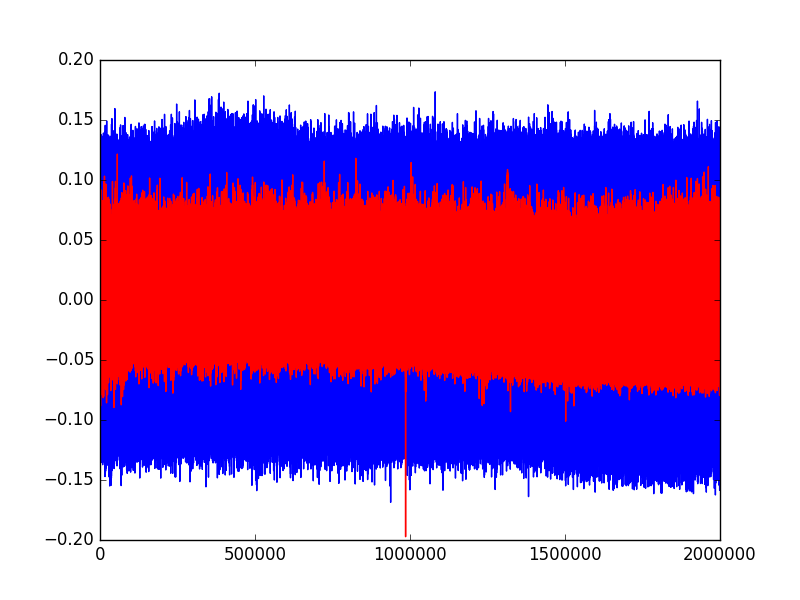
\includegraphics[scale=0.4]{figures/CPA1O_2Mpts_trickedaS+b0_1ktraces.png}
	\caption{Correlation coefficients obtained when targeting $\rmult \times Z_{\hat{\key}}[i] \oplus \rout$, for every value of $\hat{\key}$. Correct hypothesis is plotted  in red. }
	\label{fig:CPA1O_trickedaZb1}
\end{figure}

%attack_results_without_flaw_fixed_100k
\subsubsection{Multiplicatively masked Sbox output}
We suppose the knowledge of the multiplicative mask. This knowledge allows for the prediction of the value $\rmult \times Z_{\hat{\key}}[i]$ for any hypothesis $\hat{\key}$.
The attack is unsuccessful using $50.000$ traces.
Figure~\ref{fig:CPA1O_trickedaZ1} illustrates the result of the attack targeting byte 0, using $50.000$ traces.

\begin{figure}[H]
	\centering 
	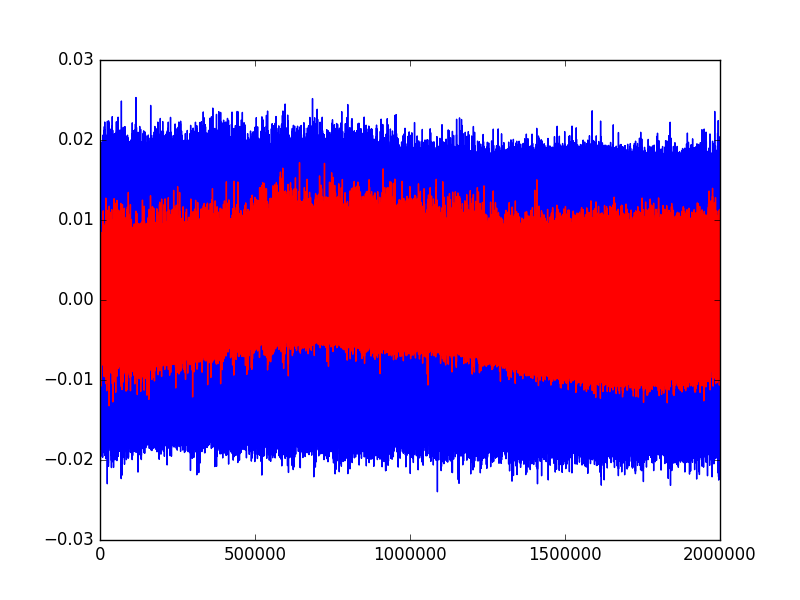
\includegraphics[scale=0.4]{figures/CPA1O_2Mpts_trickedaS0traces.png}
	\caption{Correlation coefficients obtained when targeting $\rmult \times Z_{\hat{\key}}[i]$, for every value of $\hat{\key}$. Correct hypothesis is plotted  in red. }
	\label{fig:CPA1O_trickedaZ1}
\end{figure}

%attack_results_without_flaw_fixed_100k
\subsubsection{Raw Sbox output}
We suppose no prior knowledge (except the permutation), and predict the value $Z_{\hat{\key}}[i]$ for any hypothesis $\hat{\key}$.
The attack is unsuccessful using $50.000$ traces.
Figure~\ref{fig:CPA1O_trickedZ1} illustrates the result of the attack targeting byte 0, using $50.000$ traces.

\begin{figure}[H]
	\centering 
	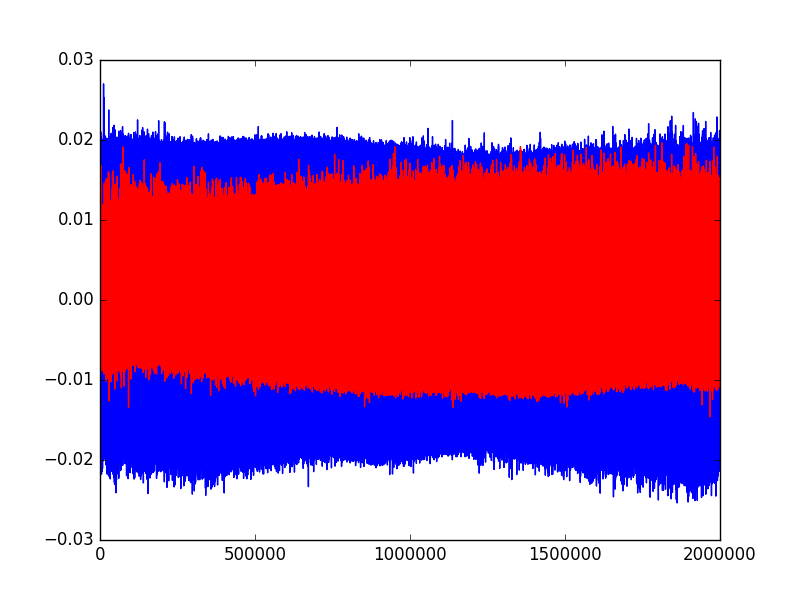
\includegraphics[scale=0.4]{figures/CPA1O_2Mpts_trickedS0traces.png}
	\caption{Correlation coefficients obtained when targeting $\rmult \times Z_{\hat{\key}}[i]$, for every value of $\hat{k}$. Correct hypothesis is plotted  in red. }
	\label{fig:CPA1O_trickedZ1}
\end{figure}

\subsection{Unknown permutation, processed traces}
We now study the setting where the attacker does not know the random masks used to compute the permutation.

We preprocess the traces in order to average the leakage over the different byte indices manipulation:
\begin{itemize}
	\item for each index $i$ in $[0,15]$, we define a small window $w_i$ of $\ell$ points around the SNR peak corresponding to the manipulation of $\rmult \times S[P[Sh(i)] \oplus K[Sh(i)]]\oplus \rout$ in the characterization phase. In our experiments, the size of the window was arbitrarily fixed to $\ell=11$.
	\item for each trace in our acquisition campaign, we compute the average window $m$ such that for each time sample $j$, $m[j]=\frac{1}{16}\sum_{i=0}^{15} w_i[j]$. We then consider $m$ as our reduced averaged trace of size $\ell$.
\end{itemize}

%/media/nas/projects/ASCAD_CW/ASCAD_ChipWhisperer/ARM/traces/averaged_attack_results_without_flaw_fixed_100k.h5
\subsubsection{Affinely masked Sbox output}
We suppose the knowledge of both the multiplicative mask and the output mask. This knowledge allows for the prediction of the value $\rmult \times S[\plain[i]\oplus \hat{\key}] \oplus \rout$ for any hypothesis $\hat{\key}$ on one byte of the secret key.
Depending on the byte index, the CPA is successful using around $20.000$ to $30.000$ traces.

Figure~\ref{fig:CPA1O_averaged_aZb1} illustrates the results using $50.000$ traces.
\begin{figure}[H]
	\centering 
	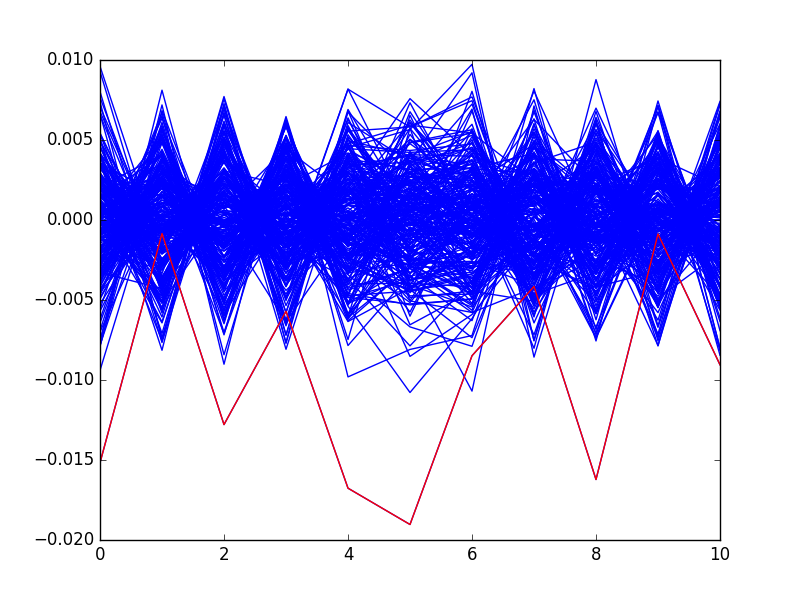
\includegraphics[scale=0.4]{figures/CPA1O_averaged_aZb1.png}
	\caption{Correlation coefficients obtained when targeting $\rmult \times S[\plain[i]\oplus \hat{\key}] \oplus \rout$, on averaged traces, for every value of $\hat{\key}$. Correct hypothesis is plotted  in red.}
	\label{fig:CPA1O_averaged_aZb1}
\end{figure}

\subsubsection{Multiplicatively masked Sbox output}
With $50.000$ traces, the attack does not succeed when targeting $\rmult \times S[\plain[i]\oplus \hat{\key}]$.
Figure~\ref{fig:CPA1O_averaged_aZ1} illustrates the results using $50.000$ traces.

Figure~\ref{fig:CPA1O_averaged_aZ1} illustrates the results using $50.000$ traces.
\begin{figure}[H]
	\centering 
	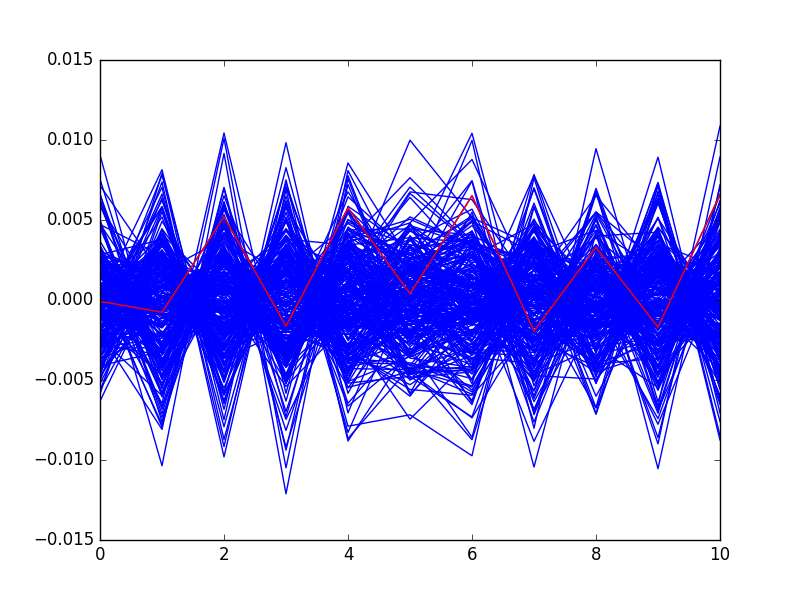
\includegraphics[scale=0.4]{figures/CPA1O_averaged_aZ1.png}
	\caption{Correlation coefficients obtained when targeting $\rmult \times S[\plain[i]\oplus \hat{\key}] \oplus \rout$, on averaged traces, for every value of $\hat{\key}$. Correct hypothesis is plotted in red.}
	\label{fig:CPA1O_averaged_aZ1}
\end{figure}


\subsubsection{Raw Sbox output}
With $50.000$ traces, the attack does not succeed when targeting $S[\plain[i]\oplus \hat{\key}]$.
Figure~\ref{fig:CPA1O_averaged_Z1} illustrates the results using $50.000$ traces.
Figure~\ref{fig:CPA1O_averaged_Z1} illustrates the results using $50.000$ traces.

\begin{figure}[H]
	\centering 
	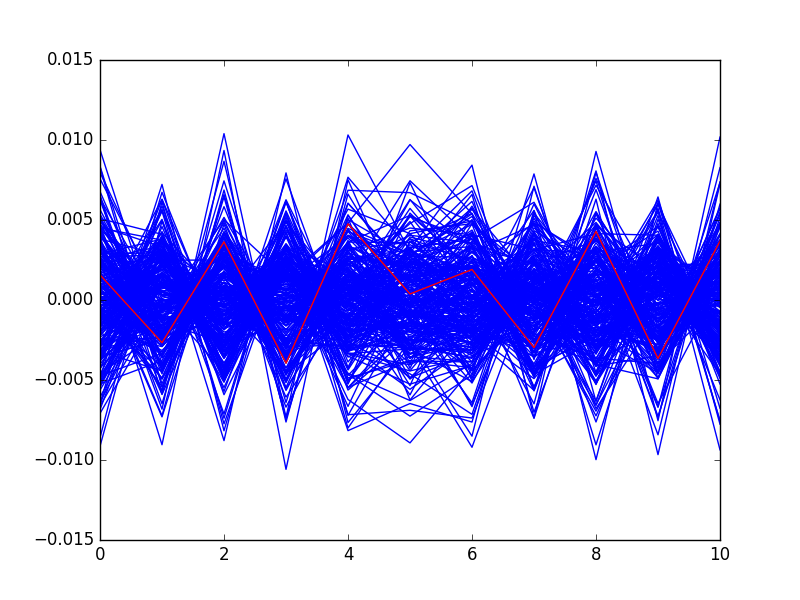
\includegraphics[scale=0.4]{figures/CPA1O_averaged_Z1.png}
	\caption{Correlation coefficients obtained when targeting $\rmult \times S[\plain[i]\oplus \hat{\key}] \oplus \rout$, on averaged traces, for every value of $\hat{\key}$. Correct hypothesis is plotted  in red.}
	\label{fig:CPA1O_averaged_Z1}
\end{figure}

\subsection{Unknown permutation, non-processed traces}

For the sake of completeness, we also perform these experiments on raw unprocessed traces. No success is obtained when targeting $Z_{\hat{\key}}[i]$ or $\rmult \times Z_{\hat{\key}}[i]$ using $50.000$ traces.
Similarly, by targeting $\rmult \times S[\plain[i]\oplus \hat{\key}] \oplus \rout$, the attack does not succeed.


\subsection{Summary}
The results in this section evidence the effectiveness of the implementation of the countermeasures against first-order side-channel attack.
Assuming knowledge of the mask values, the shuffling countermeasure alone increases the number of necessary traces by a factor $\sim 20$.
Furthermore, masking countermeasures seem to completely thwart first order side-channel attacks using $50.000$ traces.


\begin{figure}[h!]
\centering
\begin{tabular}{|c|c|c|c|c|c|c|}
  \hline
   & \multicolumn{3}{c|}{Known permutation}&\multicolumn{3}{c|}{Unknown permutation}\\
  \hline
  Known & $\rmult, \rout$ & $\rmult $ &  None & $\rmult,\rout$ & $\rmult $  &  None \\
  \hline
  \# Traces& $\approx 1.000$ & $ > 50.000$ & $> 50.000$& $\approx 20.000$ & $ > 50.000$ & > $50.000$\\
  \hline
\end{tabular}
\caption{Number of traces needed for a successful first-order attack, in the different settings.}
\end{figure}

